\section{Durchführung}
\label{sec:Durchführung}
Es wird die Apperatur aus \autoref{3} verwendet. 
\begin{figure}[H]
  \centering
  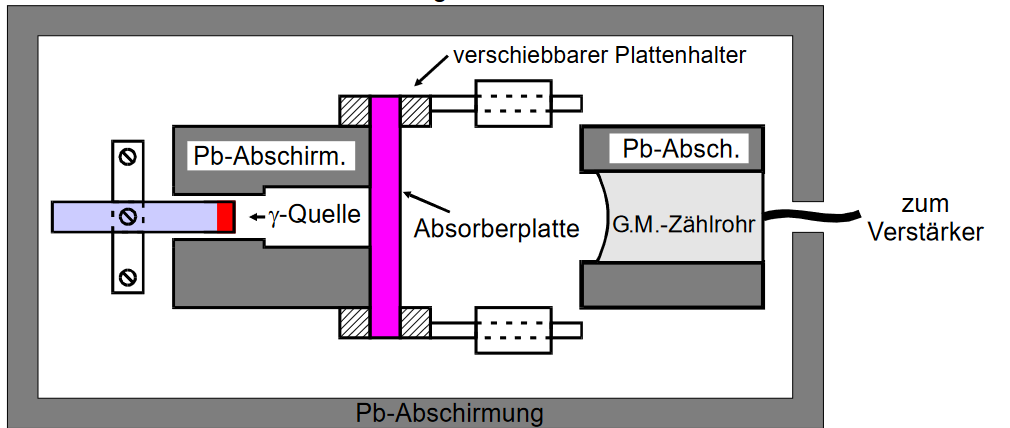
\includegraphics[width=9cm]{content/3}
  \caption{Messaufbau für den Versuch \cite{sample}.}
  \label{3}
\end{figure}
Sie besteht aus einer Halterung für den Strahler, einem Geiger-Müller-Zählrohr, einem Halter für Platten und einer Bleiabschirmung für $\gamma$-Strahlung und einer Aluminiumabschirmung für $\beta$-Strahlung. Außerdem ist der Geiger-Müller-Zähler an einem Impulsmessgerät angeschlossen.\\
Mit dem Impulsmessgerät wird ohne Strahler zu erst eine Nullmessung durchgeführt, um das Rauschen zu ermitteln. Dann werden die vorher abgemessenen Platten in die Konstruktion gelegt und die Impulsrate für die jeweiligen Strahler aufgenommen. Die Messzeit muss dabei an die Dicke angepasst werden. Für den Versuch wurde ein $^137 Cs$-Strahler und ein $^99 Tc$-Strahler verwendet.
